\documentclass[12pt]{article}


\usepackage{graphicx}
\usepackage{xepersian}
\usepackage{amsmath}
\usepackage{indentfirst}
\setlength{\parindent}{1cm}

\settextfont{Arial}


\begin{document}
	
	
	\begin{titlepage}
		
		\centering
		
		\vspace*{1cm}
		
		{\Huge \bfseries
			گزارشکار آزمایشگاه پردازش سیگنال دیجیتال
			\par}
		
		\vspace{0.7cm}
		
		{\LARGE
			آزمایش دوم
			\par}
		
		\vspace{0.5cm}
		
	
		\vspace{0.3cm}
		
		{\Large
			نویسنده: شیما محققی
			\par}
		
		\vfill
		
		{\large
			\today
			\par}
		
		
		
		\begin{figure}
			\begin{center}
				\includegraphics[width=0.65\textwidth]{download1.png}
			\end{center}
		\end{figure}
		
	\end{titlepage}
	
	
	
	
	
	
	
	\newpage
	
	\section{بخش 2-2 }
	
	\subsection{تحلیل و مقایسه سیگنال اصلی ($sn$) و سیگنال نویزی ($xn$)}
	
	در این بخش از آزمایش، به منظور بررسی اثر نویز بر سیگنال‌های مخابراتی، سیگنال مطلوب $sn$ با دو مولفه‌ی نویز فرکانس پایین و فرکانس بالا ترکیب شده است. 
	\begin{itemize}
		\item \textbf{اثر نویز فرکانس پایین ($0.05\pi$):} 
		این مولفه به دلیل داشتن فرکانس بسیار کمتر نسبت به سیگنال اصلی، باعث ایجاد یک روند (Trend) یا تغییر سطح DC متغیر در زمان شده است. در نمودار $xn$ کاملاً مشهود است که سیگنال اصلی روی این موج با فرکانس پایین سوار شده و باعث شده است که تشخیص مقدار واقعی و لحظه‌ای سیگنال $sn$ بسیار دشوار گردد.
		
		\item \textbf{اثر نویز فرکانس بالا ($0.35\pi$):} 
		این مولفه باعث ایجاد ریپل‌های (Ripple) سریع و لرزش‌های متناوب روی بدنه سیگنال اصلی شده است. این پدیده منجر به از بین رفتن همواری  نمودار $sn$ شده و در نتیجه، ویژگی‌های ظاهری سیگنال سینوسی اولیه کاملاً دفرمه شده است.
	\end{itemize}
	
	\textbf{نتیجه‌گیری:}
	این مقایسه به خوبی نشان می‌دهد که نویزهای جمع‌شونده چگونه می‌توانند پارامترهای اساسی سیگنال از جمله دامنه، فاز و شکل موج لحظه‌ای را تخریب کنند. برای بازیابی سیگنال مطلوب $sn$ از دل این سیگنال آلوده، طراحی و اعمال یک فیلتر میان‌گذر با فرکانس مرکزی $0.2\pi$ ضروری است تا بتواند هر دو مولفه‌ی مزاحم در فرکانس‌های $0.05\pi$ و $0.35\pi$ را حذف نماید.
	

	 \begin{figure}[!h]
		     \centering
		     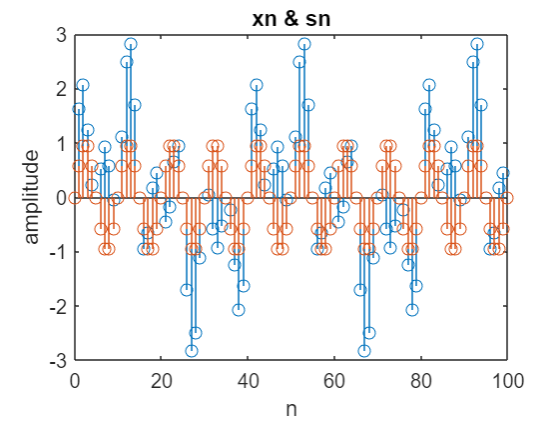
\includegraphics[width=0.7\textwidth]{Screenshot (123).png}
		     \caption{مقایسه سیگنال مطلوب و سیگنال نویزی در حوزه زمان}
		     \label{fig:part_a_comparison}
		 \end{figure}
	\newpage

	
	\subsection{تحلیل نتایج فیلترینگ و مقایسه خروجی با سیگنال مطلوب}
	در این بخش، خروجی فیلتر طراحی شده ($y[n]$) با سیگنال اصلی و بدون نویز ($s[n]$) مورد مقایسه قرار گرفته است که نتایج آن در نمودار زیر مشاهده می‌شود.
	
	\begin{itemize}
		\item \textbf{پاسخ گذرا :} 
		همان‌طور که در نمودار مشهود است، در بازه ابتدایی (تقریباً تا $n=50$)، خروجی فیلتر با سیگنال اصلی انطباق ندارد. این پدیده به دلیل خاصیت فیلترهای FIR و طول فیلتر ($M=100$) رخ می‌دهد. از آنجا که تأخیر گروهی فیلتر برابر با $\tau_g = \frac{M}{2} = 50$ نمونه است، فیلتر برای رسیدن به حالت پایدار نیاز به دریافت نمونه‌های اولیه دارد.
		
		\item \textbf{بررسی دامنه و نرمال‌سازی:}
		با اعمال ضریب تصحیح بر اساس پاسخ فرکانسی در فرکانس هدف ($\omega = 0.2\pi$)، مشاهده می‌شود که دامنه خروجی فیلتر دقیقاً بر دامنه سیگنال اصلی منطبق شده است. این امر نشان‌دهنده موفقیت در تنظیم بهره فیلتر  در باند عبور است.
		
		\item \textbf{حذف مؤلفه‌های نویز:}
		انطباق شکل موج آبی بر نارنجی پس از گذشت فاز گذرا، تأیید می‌کند که فیلتر میان‌گذر به درستی عمل کرده و توانسته است مؤلفه‌های مزاحم در فرکانس‌های $0.05\pi$ و $0.35\pi$ را به طور کامل تضعیف کند و تنها فرکانس اصلی $0.2\pi$ را عبور دهد.
	\end{itemize}
	

	\begin{figure}[!h]
		\centering
		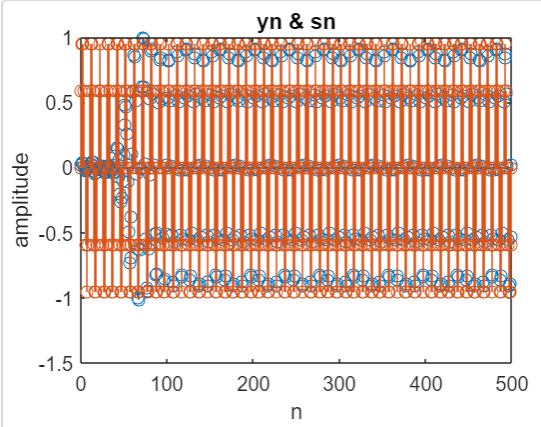
\includegraphics[width=0.7\textwidth]{Screenshot (127).png}
		\caption{مقایسه سیگنال خروجی فیلتر ($y[n]$) و سیگنال مطلوب ($s[n]$)}
		\label{fig:part_a_comparison}
	\end{figure}
	
	\newpage
	
	\subsection{تحلیل فیلترینگ سیگنال نویزی و بررسی تأخیر گروهی}
	در این مرحله، سیگنال نویزی $x[n]$ به فیلتر میان‌گذر طراحی شده اعمال گردید. با توجه به نمودارهای حاصل، موارد زیر قابل استخراج است:
	
	\begin{enumerate}
		\item \textbf{بهبود کیفیت سیگنال:} فیلتر به خوبی توانسته است نوسانات ناشی از نویزهای فرکانس بالا و پایین را حذف کرده و سیگنال اصلی با فرکانس $0.2\pi$ را استخراج کند.
		
		\item \textbf{تحلیل تأخیر فاز :} در مقایسه نمودار Filtered Signal با Original Signal، یک جابه‌جایی زمانی به سمت راست مشاهده می‌شود. این تأخیر ناشی از خاصیت فاز خطی فیلتر FIR طراحی شده است. مقدار این تأخیر که به عنوان «تأخیر گروهی» شناخته می‌شود، طبق رابطه زیر محاسبه می‌گردد:
		\[ \tau_g = \frac{M}{2} = \frac{100}{2} = 50 \text{ samples} \]
		بنابراین، خروجی فیلتر همواره با ۵۰ نمونه تأخیر نسبت به ورودی ظاهر می‌شود.
		
		\item \textbf{پاسخ گذرا در شروع:} در ابتدای نمودار خروجی، مشاهده می‌شود که سیگنال از مقدار صفر شروع شده و پس از طی شدن ۵۰ نمونه به پایداری می‌رسد. این بازه، زمان لازم برای پر شدن حافظه فیلتر (Taps) از نمونه‌های ورودی است.
	\end{enumerate}
	\begin{figure}[!h]
		\centering
		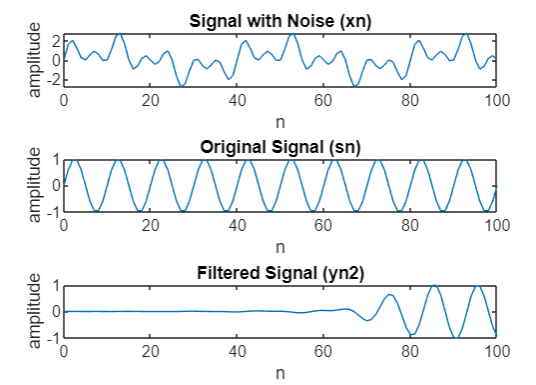
\includegraphics[width=0.7\textwidth]{Screenshot (125).png}
		\caption{تحلیل زمانی فرآیند فیلترینگ: (الف) سیگنال نویزی $x[n]$، (ب) سیگنال اصلی $s[n]$ و (ج) خروجی فیلتر شده $y[n]$ با مشاهده تأخیر گروهی.}
		
		\label{fig:part_a_comparison}
	\end{figure}
	
	\newpage
	
	\section{بخش 2-4 }
	
	
	
	در این آزمایش سیگنال مورد بررسی ترکیبی از سه مؤلفه زیر است:
	
	\begin{itemize}
		\item یک سیگنال سینوسی با فرکانس $f_0 = 100$ 
		\item یک سیگنال \lr{Chirp} خطی با تغییر فرکانس از $400$  به $200$  در بازه زمانی $[0,2]$
		\item یک ضربه با دامنه $50$ در نمونه $250$
	\end{itemize}
	
	فرکانس نمونه‌برداری سیگنال برابر با $f_s = 500$  در نظر گرفته شده است.
	
	\subsection{تحلیل خروجی FFT}
	
	تبدیل فوریه گسسته (FFT) طیف کلی سیگنال را در حوزه فرکانس نمایش می‌دهد. در خروجی FFT مشاهده می‌شود که:
	
	\begin{itemize}
		\item مؤلفه سینوسی $100$  به صورت یک قله مشخص در طیف ظاهر می‌شود.
		\item سیگنال \lr{Chirp} به دلیل تغییر فرکانس در طول زمان، انرژی خود را در بازه‌ای از فرکانس‌ها (بین $200$ تا $400$ ) پخش می‌کند.
		\item ضربه زمانی به دلیل موضعی بودن شدید در حوزه زمان، طیفی پهن‌باند در حوزه فرکانس ایجاد می‌کند.
	\end{itemize}
	
	نکته مهم آن است که FFT تنها توزیع کلی انرژی سیگنال در حوزه فرکانس را نشان می‌دهد و هیچ اطلاعاتی درباره زمان وقوع هر مؤلفه ارائه نمی‌دهد. به عبارت دیگر، اگر یک مؤلفه فرکانسی فقط در بخشی از سیگنال حضور داشته باشد، FFT قادر به مشخص کردن زمان وقوع آن نخواهد بود.
	
	بنابراین برای سیگنال‌های غیرایستا مانند سیگنال حاضر، FFT اطلاعات زمانی را از بین می‌برد و تنها یک تصویر کلی از محتویات فرکانسی ارائه می‌دهد.
	
	\subsection{تحلیل تبدیل فوریه زمان کوتاه (STFT)}
	
	برای بررسی تغییرات فرکانسی در طول زمان از تبدیل فوریه زمان کوتاه استفاده شد. در این روش سیگنال به پنجره‌های زمانی کوتاه تقسیم شده و از هر بخش یک FFT محاسبه می‌شود. خروجی این فرآیند به صورت \lr{Spectrogram} نمایش داده می‌شود که دارای دو محور زمان و فرکانس است.
	
	در نمودار اسپکتروگرام:
	
	\begin{itemize}
		\item مؤلفه سینوسی $100$  به صورت یک نوار افقی تقریباً ثابت دیده می‌شود.
		\item سیگنال \lr{Chirp} به صورت یک مسیر مورب نزولی از $400$  به $200$  مشاهده می‌شود که نشان‌دهنده کاهش تدریجی فرکانس در زمان است.
		\item ضربه در یک لحظه زمانی خاص به صورت یک ناحیه متمرکز زمانی با گستره فرکانسی زیاد ظاهر می‌شود.
	\end{itemize}
	
	بنابراین STFT علاوه بر اطلاعات فرکانسی، اطلاعات زمانی نیز ارائه می‌دهد و برای تحلیل سیگنال‌های غیرایستا بسیار مناسب‌تر از FFT است.
	
	\subsection{اثر طول پنجره بر رزولوشن زمان و فرکانس}
	
	در این آزمایش از پنجره \lr{Hamming} با طول‌های $256$ و $512$ نمونه استفاده شد.
	
	رابطه تقریبی بین طول پنجره و تفکیک‌پذیری فرکانسی به صورت زیر است:
	
	\[
	\Delta f \propto \frac{1}{N}
	\]
	
	که در آن $N$ طول پنجره است.
	
	\begin{itemize}
		\item برای $N = 256$:
		\begin{itemize}
			\item رزولوشن زمانی بهتر
			\item رزولوشن فرکانسی ضعیف‌تر
		\end{itemize}
		
		\item برای $N = 512$:
		\begin{itemize}
			\item رزولوشن زمانی ضعیف‌تر
			\item رزولوشن فرکانسی بهتر
		\end{itemize}
	\end{itemize}
	
	بنابراین بین رزولوشن زمانی و رزولوشن فرکانسی یک مبادله (Trade-off) وجود دارد و هیچ‌یک از این دو حالت به طور مطلق برتر نیست. انتخاب طول پنجره به هدف تحلیل بستگی دارد. اگر هدف بررسی تغییرات سریع زمانی مانند محل دقیق ضربه باشد، پنجره کوتاه‌تر مناسب‌تر است؛ اما اگر هدف تفکیک دقیق‌تر فرکانس‌ها باشد، پنجره بلندتر عملکرد بهتری دارد.
	\newpage
		\begin{figure}[!h]
		\makebox[\textwidth][c]{%
			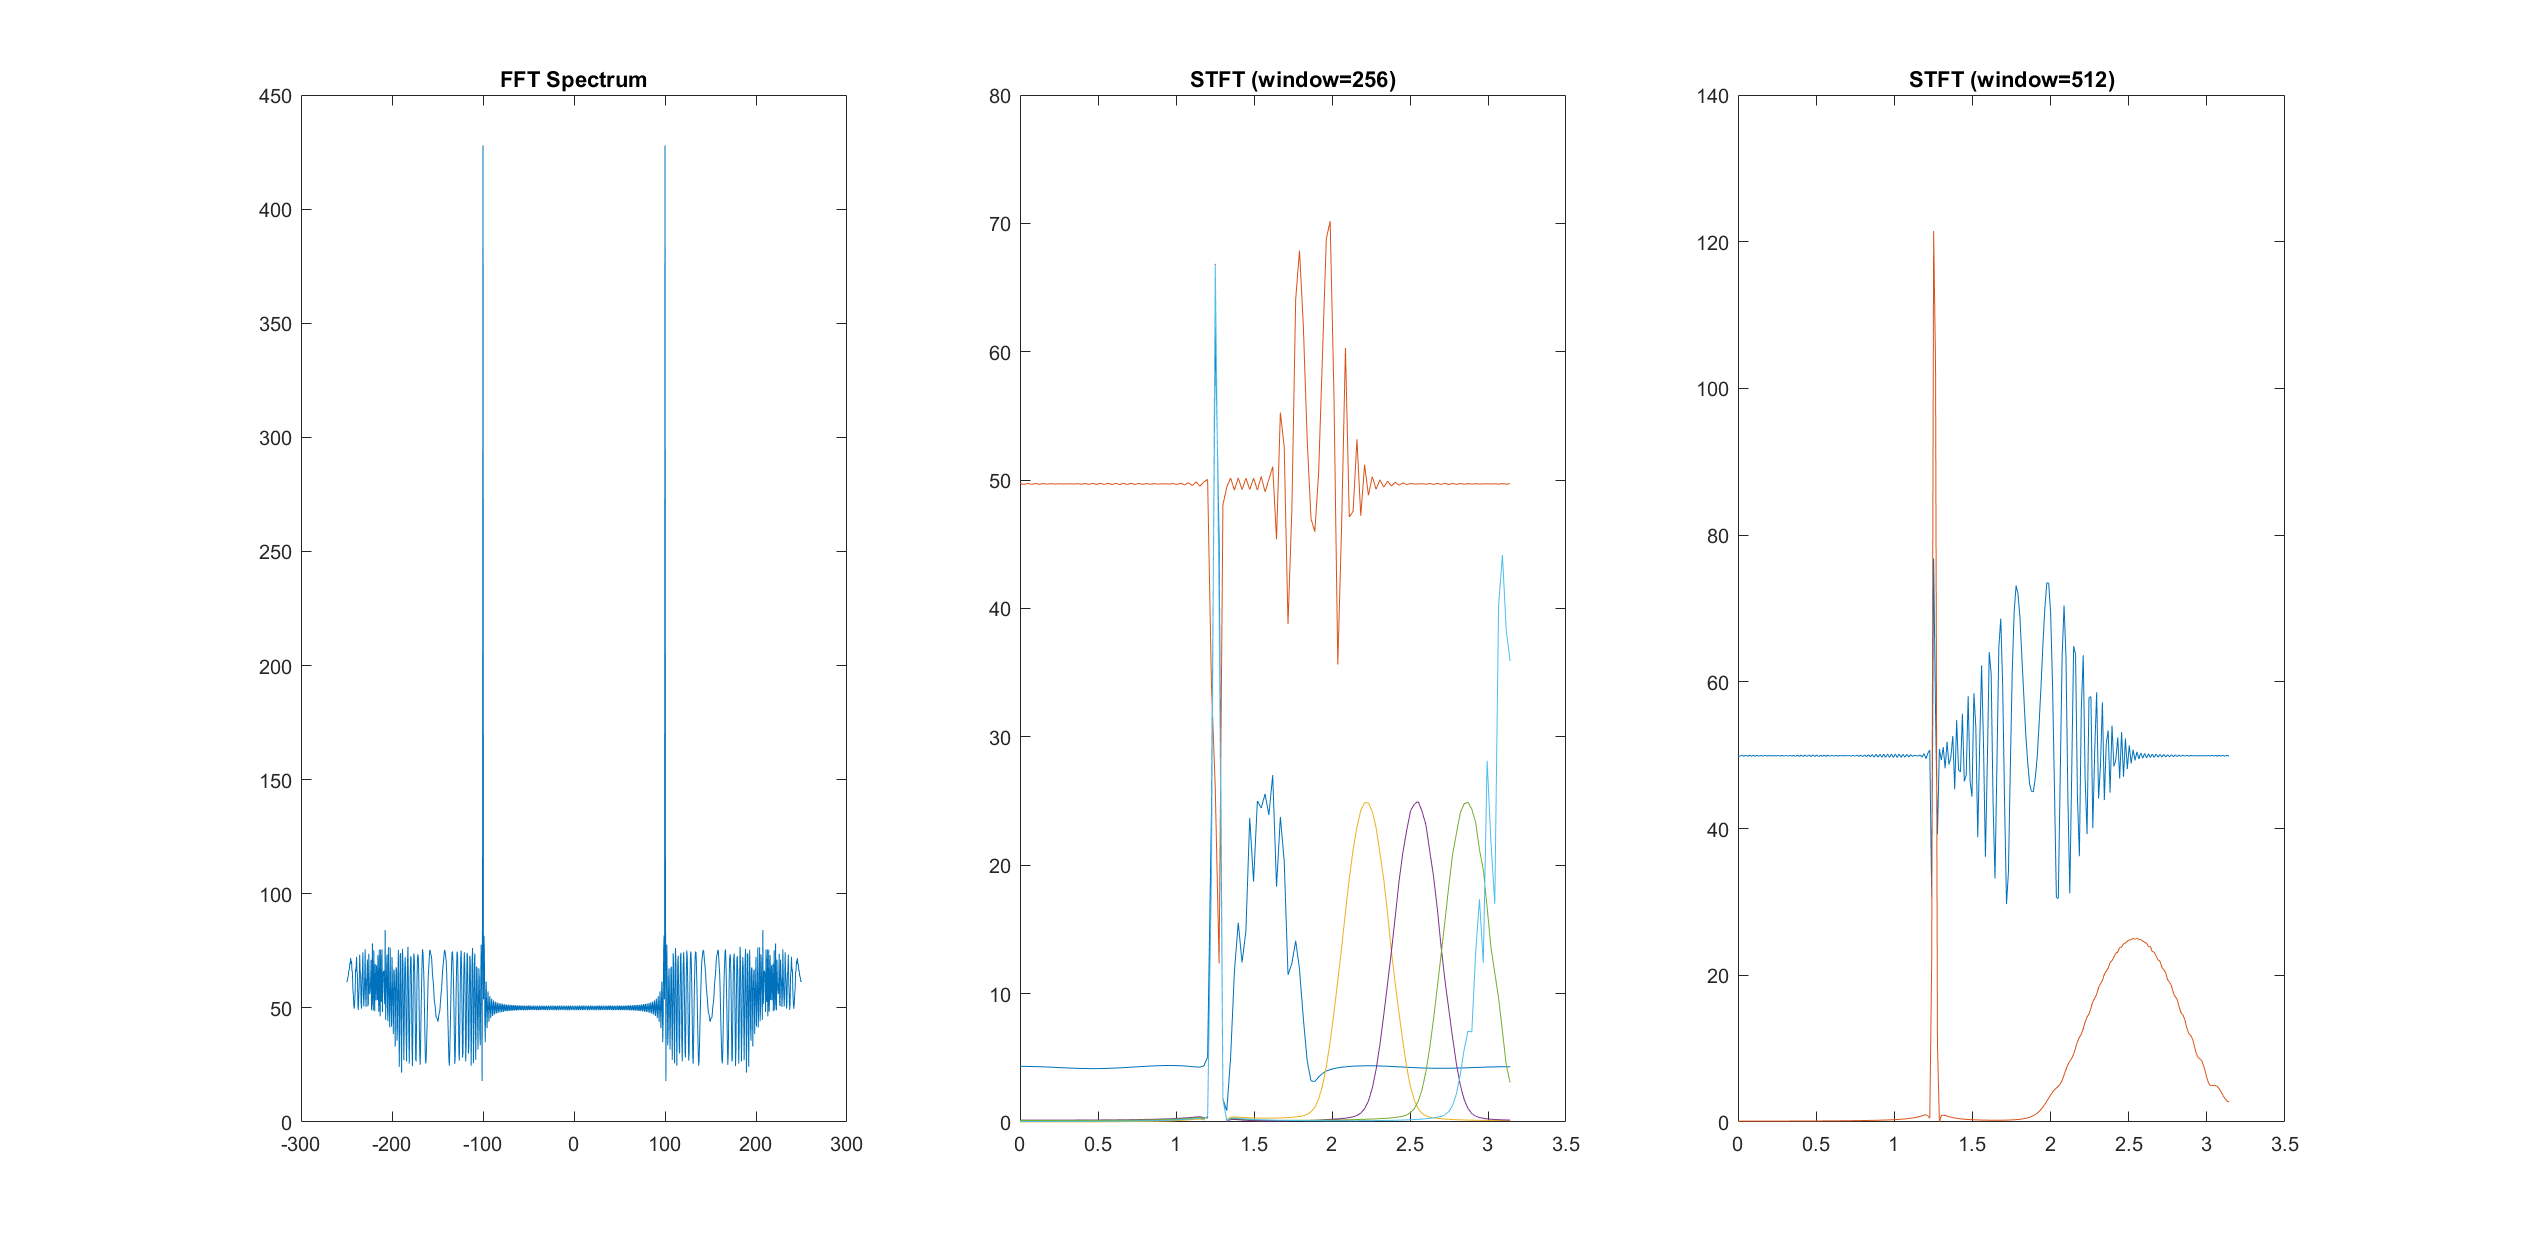
\includegraphics[width=1.3\textwidth]{Screenshot (134).png}
		}
		
		
		\caption{نتایج تحلیل سیگنال ترکیبی شامل مؤلفه سینوسی، Chirp و ضربه. (الف) طیف فرکانسی سیگنال با استفاده از FFT، (ب) اسپکتروگرام با پنجره 256 نمونه، و (ج) اسپکتروگرام با پنجره 512 نمونه.}
		\label{fig:part_a_comparison}
	\end{figure}
	
	
	\subsection{نتیجه‌گیری}
	
	نتایج نشان می‌دهد که FFT تنها تصویر کلی از طیف فرکانسی سیگنال ارائه می‌دهد و برای سیگنال‌های غیرایستا اطلاعات زمانی را از دست می‌دهد. در مقابل، STFT با نمایش همزمان اطلاعات زمان و فرکانس، امکان مشاهده تغییرات فرکانسی در طول زمان را فراهم می‌کند. به همین دلیل استفاده از اسپکتروگرام برای تحلیل سیگنال‌های شامل \lr{Chirp} و ضربه ضروری و منطقی است.
\newpage
	\section{بخش 2-5}
	

	
	یکی از محدودیت‌های اصلی تبدیل فوریه زمان-کوتاه (\lr{STFT})، ثابت بودن طول پنجره تحلیل است که طبق اصل عدم قطعیت هایزنبرگ، منجر به ایجاد رزولوشن ثابت در تمام فرکانس‌ها می‌شود. تبدیل موجک برای رفع این مشکل، از پنجره‌هایی با طول متغیر استفاده می‌کند.
	
	\subsection{مفهوم تحلیل چندرزولوشنی (\lr{MRA})}
	تبدیل موجک سیگنال را به مجموعه‌ای از توابع پایه به نام «موجک مادر» (\lr{Mother Wavelet}) منتقل می‌کند. این تبدیل با دو پارامتر اصلی کار می‌کند:
	\begin{itemize}
		\item \textbf{مقیاس (\lr{Scale}):} که معادل معکوس فرکانس است. مقیاس‌های بزرگ (پنجره‌های پهن) برای استخراج کلیات سیگنال (\lr{Approximations}) و مقیاس‌های کوچک (پنجره‌های فشرده) برای استخراج جزئیات (\lr{Details}) به کار می‌روند.
		\item \textbf{انتقال (\lr{Translation}):} که مکان موجک را در طول زمان جابه‌جا می‌کند.
	\end{itemize}
	
	\subsection{تبدیل موجک گسسته (\lr{DWT}) و ساختار درختی}
	در پردازش سیگنال دیجیتال، از \lr{DWT} استفاده می‌شود که سیگنال را از طریق یک بانک فیلتر عبور می‌دهد. در هر مرحله تجزیه:
	\begin{enumerate}
		\item سیگنال از یک \textbf{فیلتر پایین‌گذر (\lr{LPF})} عبور کرده و ضرایب \textbf{\lr{Approximation} ($A$)} حاصل می‌شوند که شامل هویت اصلی و فرکانس‌های پایین سیگنال است.
		\item سیگنال از یک \textbf{فیلتر بالاگذر (\lr{HPF})} عبور کرده و ضرایب \textbf{\lr{Detail} ($D$)} حاصل می‌شوند که شامل نویز و تغییرات سریع سیگنال است.
		\item پس از هر مرحله، عمل  کاهش نرخ نمونه‌برداری (\lr{Downsampling}) با ضریب ۲ انجام می‌شود تا حجم محاسبات بهینه بماند.
	\end{enumerate}
	
	این ساختار درختی اجازه می‌دهد تا در فرکانس‌های پایین (که معمولاً سیگنال زمان طولانی‌تری دارد) رزولوشن فرکانسی بالا، و در فرکانس‌های بالا (تغییرات سریع) رزولوشن زمانی بالایی داشته باشیم.
	
	
	در این بخش، سیگنال تست \lr{Doppler} که دارای ویژگی غیرایستا (تغییر فرکانس در زمان) است، با نویز ترکیب شده و سپس توسط تبدیل موجک گسسته با استفاده از موجک مادر \lr{sym4} مورد تحلیل قرار گرفته است.
	\newpage
	\begin{figure}[!h]
		\centering
		\includegraphics[width=0.95\textwidth]{Screenshot (135).png}
		\caption{تحلیل چندرزولوشنی سیگنال داپلر نویزی در سه سطح تجزیه.}
		\label{fig:wavelet_analysis}
	\end{figure}
	
	مطابق شکل \ref{fig:wavelet_analysis}، نتایج زیر حاصل شده است:
	
	\begin{enumerate}
		\item \textbf{نمودار اول:} سیگنال اصلی در کنار سیگنال نویزی قرار دارد. نویز موجود دارای ماهیت فرکانس بالا است که باعث زبری نمودار شده است.
		\item \textbf{نمودار دوم (سطح ۱):} با حذف اولین سطح از ضرایب جزئیات (\lr{Detail})، نویزهای با فرکانس بسیار بالا حذف شده و سیگنال کمی نرم‌تر شده است.
		\item \textbf{نمودار سوم (سطح ۲):} در این مرحله انطباق سیگنال بازسازی شده بر سیگنال اصلی بسیار بیشتر شده و بخش بزرگی از نویز حذف گردیده است.
		\item \textbf{نمودار چهارم (سطح ۳):} در این سطح، سیگنال بسیار نرم شده است؛ اما مشاهده می‌شود که در ابتدای سیگنال (سمت چپ) که فرکانس نوسانات سیگنال اصلی بالاست، فیلتر موجک بخشی از اطلاعات اصلی سیگنال را نیز به عنوان نویز حذف کرده و باعث ایجاد اعوجاج شده است.
	\end{enumerate}
	
	\textbf{نتیجه‌گیری:} تبدیل موجک ابزاری قدرتمند برای حذف نویز از سیگنال‌های غیرایستا است، اما انتخاب سطح تجزیه (\lr{Decomposition Level}) باید به گونه‌ای باشد که از حذف اطلاعات اصلی سیگنال جلوگیری شود.
	
\end{document}